%%%%%%%%%%%%%%%%%%%%%%%%%%%%%%%%%%%%%%%%%%%%%%%%%%%%%%%%%%%
% --------------------------------------------------------
%  ____  _           
% |  _ \| |__   ___  
% | |_) | '_ \ / _ \ 
% |  _ <| | | | (_) |
% |_| \_\_| |_|\___/ 
%
% LaTeX2e Template
% Version 3.0.0 (24/02/2026)
%
% Author: 
% Guillermo Jimenez (memo.notess1@gmail.com)
% 
% Contributor:
% Eduardo Gracidas (eduardo.gracidas29@gmail.com)
%
% License:
% Creative Commons CC BY 4.0
% --------------------------------------------------------
%%%%%%%%%%%%%%%%%%%%%%%%%%%%%%%%%%%%%%%%%%%%%%%%%%%%%%%%%%%
% --------------------------------------------------------
% Find the latest version on GitHub:
% https://github.com/MemoJimenez/Rho-class
% --------------------------------------------------------
%%%%%%%%%%%%%%%%%%%%%%%%%%%%%%%%%%%%%%%%%%%%%%%%%%%%%%%%%%%

\documentclass[9pt,a4paper,twocolumn,twoside]{rho-class/rho}

\usepackage{xurl} % 放在导言区
\usepackage{siunitx} % 处理表格中的S列对齐
\usepackage{rho-class/rhoenvs}
\usepackage{rho-class/rhobabel}
\urlstyle{tt}      % 设置为等宽字体


% 重新定义你的命令
\providecommand{\inlinecode}[1]{#1}
\renewcommand{\inlinecode}[1]{%
    \begingroup
    \setlength{\fboxsep}{1.5pt}%
    \colorbox{gray!15}{\texttt{\detokenize{#1}}}%
    \endgroup
}

% CJK support for Chinese text in the document
%\usepackage{ctex}

% Fallbacks for older TeX kernels that lack tagging commands
\providecommand\taggingSocket[1]{}
\providecommand\UseTaggingSocket[1]{}
\providecommand\SuspendTagging[1]{}
\providecommand\ResumeTagging[1]{}

% Fallbacks if language labels are not defined
\providecommand{\andlanguage}{ and }
\providecommand{\keywordname}{\textbf{Keywords: }}


%% Spanish babel recomendation
% \usepackage[spanish,es-nodecimaldot,es-noindentfirst]{babel}

%----------------------------------------------------------
% Title
%----------------------------------------------------------

\doctype{POLI 3148 Final Project Report}
\title{Loyalty Signalling in Hong Kong: A Textual Analysis of Political Discourse from 1997 to 2026}

%----------------------------------------------------------
% Authors, Affiliations and dates
%----------------------------------------------------------

\author[{\textasteriskcentered},a, 1]{Deng, Xinran}
\author[{\textdagger},b,2]{Liu, Jingyi}
\author[{\textdagger},c,3]{Zhong, Jingquan}

%----------------------------------------------------------

\affil[a]{The University of Hong Kong}
\affil[b]{The University of Hong Kong}
\affil[c]{The University of Hong Kong}

%----------------------------------------------------------

\dates{This manuscript was compiled on \today.}

%----------------------------------------------------------
% Corresponding author-, Document- information
%----------------------------------------------------------

%\corres{\textsuperscript{\textasteriskcentered}Corresponding author: \href{mailto:author.one@institute.org}{author.one@institute.org} (A. One).}
%\corres{\textsuperscript{\textdagger}These authors contributed equally to this work.}

%----------------------------------------------------------

\docinfo{Template by Guillermo Jimenez, licensed under Creative Commons BY 4.0. Adapted by the authors for this research report.} 

%----------------------------------------------------------

%\journalname{LATEX}
%\journal{Rho-class (v.3) 2026}
%\theday{\today}
%\vol{X}
%\no{X}

%----------------------------------------------------------
% Abstract and Keywords
%----------------------------------------------------------

\begin{abstract}
    This paper investigates the evolution of “loyalty signaling“ by Hong Kong Chief Executives (CEs) toward the central government. While the definition of “loyalty” remains conceptually fluid and vague in Chinese politics, we propose a six-dimensional framework to categorize how political alignment is communicated. And the authors quantify the frequency of loyalty signaling by CEs through two proxies: (i) loyalty keywords density in speeches and press releases, and (ii) the semantic similarity between the speeches of CEs and central leaders. By analyzing the temporal trend in loyalty signaling from 1997 to 2026, this paper reveals a distinct cyclical pattern: loyalty signaling intensifies following periods of socio-political friction or ”trust crises” between Hong Kong and the Central Government. The results suggest that loyalty signaling is a reparative strategy directed to regain political confidence and signal political alignment during times of uncertainty. Notably, despite a surge in loyalty-signaling keyword density over the past decade, empirical evidence does not support the hypothesis of a growing convergence in political discourse between Hong Kong and Mainland China. 
    
\end{abstract}

%----------------------------------------------------------

\keywords{loyalty signaling, political discourse, central-local relations, text mining}

%----------------------------------------------------------
\renewcommand{\andlanguage}{ and } % Fix spanish y issue

\begin{document}

    \maketitle
    \thispagestyle{firststyle}

%----------------------------------------------------------

\section{Introduction}

    \rhostart{L}oyalty signaling is blablablablablablabla blabl blablablabla ablablablablab blablablabla

    \hl{insert words here}
	
    
    \subsection{Literature Review}

        \hl{insert words here}

\section{Methodology}

    \subsection{Data Collection}
    
               
        The primary dataset consists of a corpus containing Traditional Chinese government official press releases (6994 in total) and CE speeches and articles (2697 in total). 
        The fetched data spans five administrative terms (July 1997 to March 2026), capturing official discourse from Tung Chee-hwa, Donald Tsang, Leung Chun-ying, Carrie Lam, 
        and John Lee.\footnote{Press release for current administration (Traditional Chinese) can be found at: \url{https://www.ceo.gov.hk/tc/press.html}; 
        CE speeches: \url{https://www.ceo.gov.hk/tc/speeches.html}; Archive of past CE's speeches and press releases:\url{https://www.ceo.gov.hk/tc/links.html}}
        
        
        The central leaders’ addresses about Hong Kong are collected as the proxy for Mainland political discourse.\footnote{Data regarding central leaders' speeches about 
        Hong Kong was accessed from the Liaison Office of the Central People's Government (LOCPG) website: \url{http://www.locpg.gov.cn/zxzx/zysy.htm}. But the dataset is 
        restrained to the period from 2008 to 2026.} This paper studies the similarity between central leader addresses and CE speeches to assess the degree of rhetorical 
        alignment and convergence of political discourse between Mainland and Hong Kong.

            



    \subsection{Conceptualizing 'Loyalty Signaling'}

        \hl{insert words here}

    \subsection{Keyword Detection}

		The data cleaning phase involved adjusting character encoding for the accurate rendering of Traditional Chinese characters, handling missing values, and stripping HTML tags, punctuation, and extraneous whitespace. A length threshold was enforced, excluding any documents with fewer than 2,000 characters. Additionally, temporal metadata was standardized by extracting publication years via regular expressions and formatting dates to DD-MM-YYYY, restricting the analytical window strictly to the 1997–2026 period.
        
        Data wrangling procedures include transforming the unstructured corpus into structured DataFrames for quantitative analysis, and conducting text normalization and stop word removal to prepare the text for subsequent processing.

        The following computational steps are performed to transform raw text into measurable density metrics:
        
        \begin{itemize}
            \item Temporal categorization: a regular expression function, \inlinecode{extract\_year}, was used to identify the year of publication from the file names.
            \item Keyword extraction: for every document, the script iterated through the dictionary and counted the total occurrences (Hits) of every defined keyword.
            \item Normalization and density metrics: to account for varying document lengths, the \textit{Loyalty Signaling Keyword Density} was calculated using the following formula:
            
            \begin{equation}
                \text{Density} = \left( \frac{\sum \text{Keyword Hits}}{\text{Total Character Count}} \right) \times 10,000
            \end{equation}
            
            This normalization yields a standardized metric representing keyword frequency per 10,000 characters, allowing for a statistically valid longitudinal comparison across the dataset.
            
        \end{itemize}


	\subsection{Cosine Similarity Analysis}

        CE speeches and Hong Kong-related discourse from Mainland Chinese leaders are parsed using regular expressions to extract publication dates and categorized into annual corpora. 
        The raw text undergoes rigorous cleaning, including the removal of non-Chinese characters and HTML tags. The \inlinecode{jieba} library is used for precise Chinese semantic segmentation.

        To isolate "loyalty signaling" from routine administrative language, loyalty keyword boosting and customized stop-word filter are implemented. The TF-IDF algorithm is implemented to 
        transform unstructured text into high-dimensional numerical vectors. The model utilizes a \inlinecode{max_df} of 0.85 and a \inlinecode{min_df} of 2 to remove extremely common or statistically insignificant tokens.

        The degree of discursive convergence is quantified using Cosine Similarity.
        \begin{equation}
            \text{Cosine Similarity} = \frac{\mathbf{A} \cdot \mathbf{B}}{\|\mathbf{A}\| \|\mathbf{B}\|}
        \end{equation}
       
        where $\mathbf{A}$ and $\mathbf{B}$ represent the TF-IDF vectors of CE speeches and central leader addresses, respectively. This metric ranges from 0 (completely dissimilar) to 1 (identical), providing a quantitative 
        measure of rhetorical alignment over time.
        

\section{Results and Findings}

    \subsection{Loyalty Signaling in CE Speeches}

        The density of loyalty-signaling keywords in Chief Executives’ speeches varied significantly across administrations (ANOVA result: F(4,2692) = 558.02, p < .001). Tung established a moderate 
        baseline for loyalty rhetoric, which remained relatively stable throughout his tenure, marked by a slight uptick preceding his resignation. Following Tung, loyalty signaling plummeted. For 
        both Tsang and Leung, the median keyword density dropped to zero, indicating that in at least half of their analyzed speeches, loyalty keywords did not appear a single time. Although Figure 1 
        shows a visual upward trend in signaling at the end of Leung’s term, statistical analysis demonstrates no significant difference in the overall signaling density between Tsang and Leung.
            
        A dramatic escalation in loyalty signaling occurred during Carrie Lam’s administration. The frequency climbed steadily from 2017, reaching its peak in 2020. Her mean signaling density was 
        more than double that of Tung's and nearly five times higher than Leung’s. This rhetorical shift reached its absolute triumph under John Lee’s administration. Not only is his keyword density 
        the highest, his lowest Coefficient of Variation (CV) further suggests that his high volume of loyalty signaling is not isolated to specific events; it is a standardized, highly consistent, 
        and baked-in component of his everyday executive discourse.

        
        \begin{figure}[H]
            \centering
            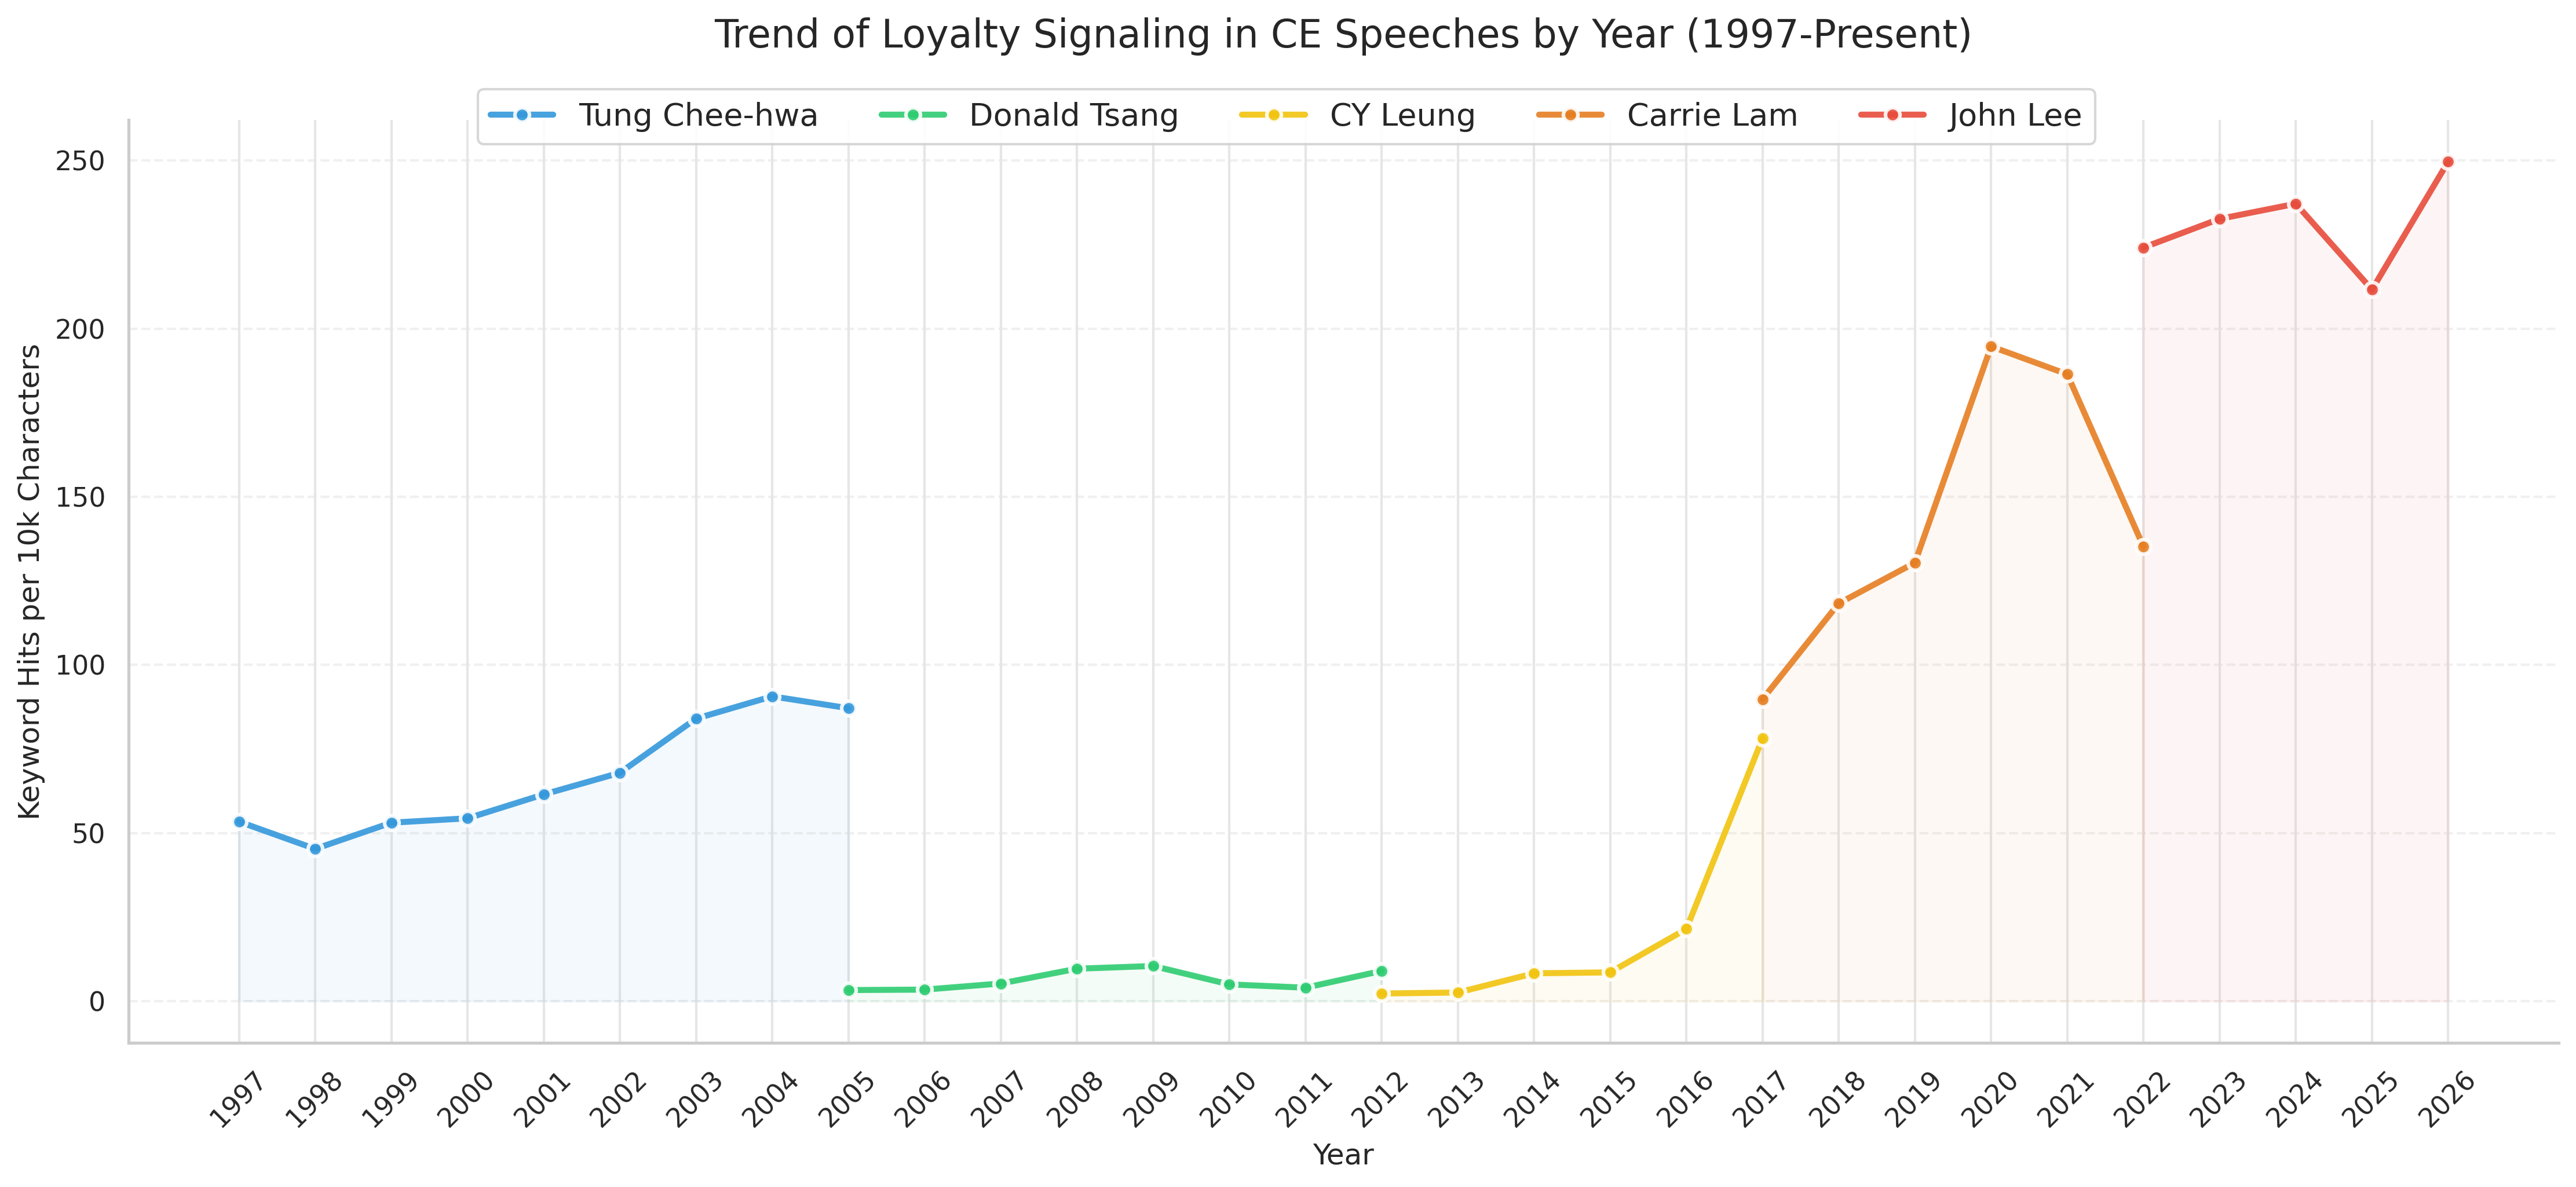
\includegraphics[width=1\columnwidth]{figures/speeches_yearly_trend.png}
            \caption{Density of loyalty-signaling keywords across administrations.}
            \label{fig:keyword_density}
        \end{figure}

        \begin{table}[ht]
            \centering
            \caption{Statistical Summary and Pairwise Comparison of Loyalty Keyword Density in CE Speeches}
            \label{tab:ce_stats}
            \small
            \setlength{\tabcolsep}{5pt} % 列间距
            \begin{tabular}{@{} l r S[table-format=3.2] S[table-format=3.2] S[table-format=1.2] c c c c @{}}
            \toprule
            & & \multicolumn{3}{c}{Descriptive Statistics} & \multicolumn{4}{c}{Post-hoc Comparison ($p$-adj)} \\
            \cmidrule(lr){3-5} \cmidrule(lr){6-9}
            CE & {$n$} & {Mean} & {Median} & {CV} & {Tung} & {Tsang} & {Leung} & {Lam} \\
            \midrule
            Tung & $497$ & 61.15  & 50.98  & 0.84 & ---     & ---  & ---  & --- \\
            Tsang  & $396$ & 16.20  & 0.00   & 2.51 & ***     & ---  & ---  & --- \\
            Leung      & $451$ & 29.41  & 0.00   & 1.74 & ***     & $.20$ & ---  & --- \\
            Lam    & $646$ & 139.93 & 112.40 & 0.76 & ***     & ***  & ***  & --- \\
            Lee      & $707$ & 228.80 & 211.60 & 0.56 & ***     & ***  & ***  & *** \\
            \bottomrule
            \addlinespace
            \multicolumn{9}{l}{\textit{Note.} Overall ANOVA: $F(4, 2692) = 558.02, p < .001$.} \\
            \multicolumn{9}{l}{*** $p < .001$; ** $p < .01$; * $p < .05$.} \\
            \end{tabular}
        \end{table}

        Chronologically, the year of 2015 serves as a critical inflection point, representing the immediate rhetorical response to the 2014 Umbrella Movement. This shift was preceded by the State 
        Council’s June 2014 White Paper, which systemically introduced the doctrine of "Comprehensive Jurisdiction" for the first time.\footnote {See \url{https://www.hmo.gov.cn/xwzx/zwyw/202312/t20231208_38591.html}
        {This document} signaled Beijing’s dissatisfaction with the local administration’s perceived inability to manage the precursors to "Occupy Central," emphasizing that Hong Kong’s autonomy is a delegated 
        power rather than an inherent right.} This trajectory of intensified signaling reached its peak in 2020, following the Anti-Extradition Law Amendment Bill Movement . While the promulgation of the National 
        Security Law (NSL) in 2020 was followed by a temporary dip in signaling density, the intensity subsequently surged to an all-time high during John Lee’s administration. These patterns strongly support the 
        conclusion that loyalty signaling in the HKSAR is most acute during periods of peak political uncertainty and serves as a reparative mechanism to restore central-local confidence.

        While the overall trend for "loyalty signaling" shows a statistically significant increase during the tenures of Carrie Lam and John Lee, this pattern is not uniform across all categories. First of 
        all, there is no rhetorical loyalty signaling throughout all the periods. Secondly, ideological loyalty has constantly remained the most dominant category in terms of absolute volume, reaching a density of 
        120.4 per 10,000 characters in Lee’s administration. But it shall be noted that Tung Chee-hwa also exhibited a high propensity for ideological signaling; as the first Chief Executive, he had to frequently 
        articulate the relationship between the HKSAR and the mainland’s socialist system. Thirdly, none of the five CEs demonstrated a significant enthusiasm for "personal loyalty" signaling, indicating that 
        political alignment in the HKSAR is projected as an institutional or systemic commitment rather than an individual allegiance. 

        \begin{figure}[H]
            \centering
            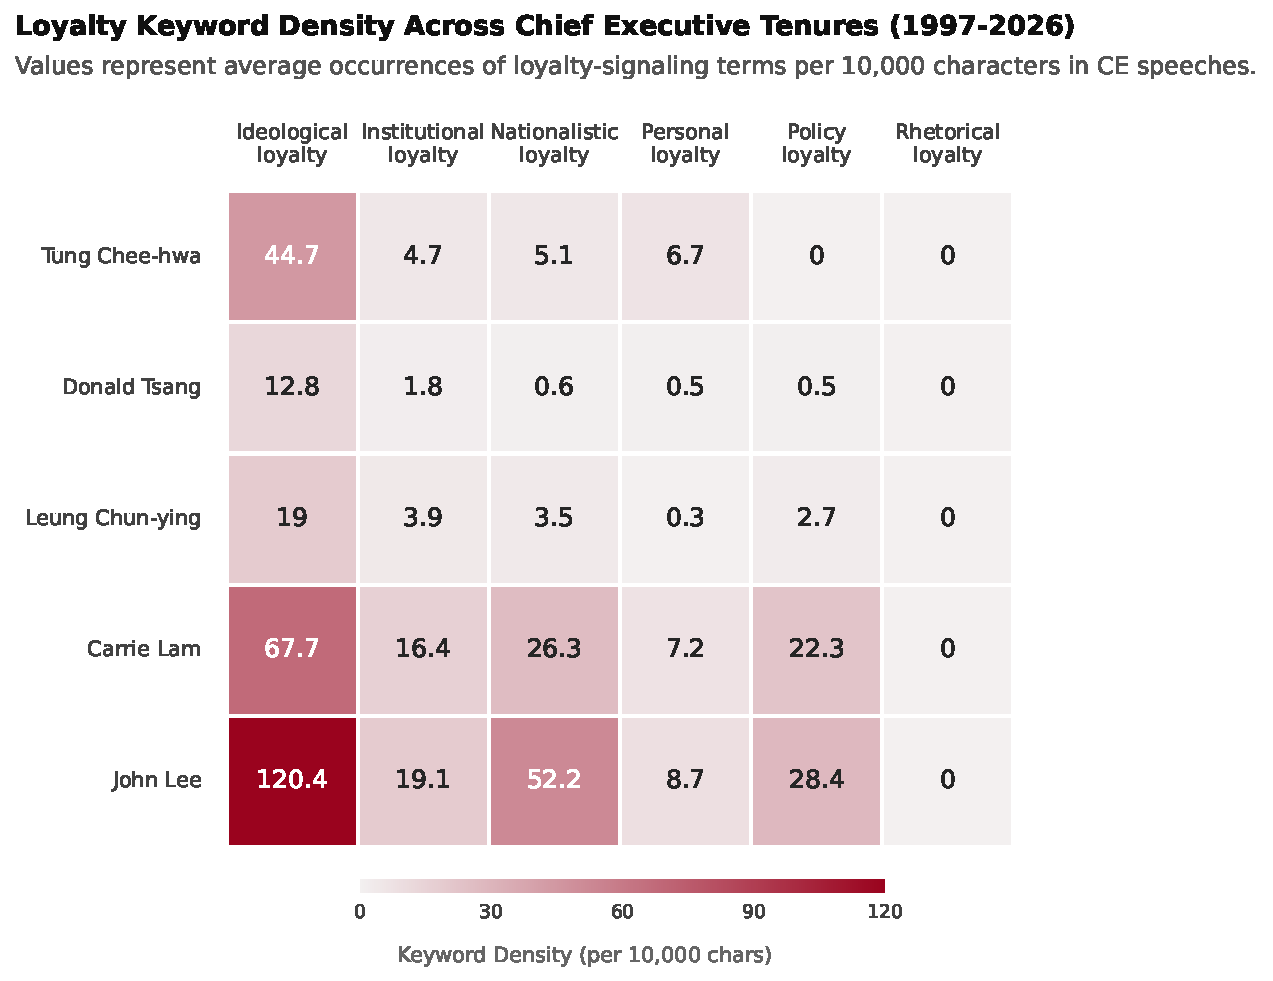
\includegraphics[width=1\columnwidth]{figures/heatmap_loyalty_sequential.pdf}
            \caption{Density of loyalty-signaling keywords by category across administrations.}
            \label{fig:category_trend}
        \end{figure}


    \subsection{Loyalty Signaling in Press Releases}

        For Tung Chee-hwa, Carrie Lam, and John Lee, there is a statistically significant difference (p< .001) between their spoken speeches and written press releases. In all three cases, they deploy vastly 
        more loyalty signaling through spoken words than in press releases. Whereas for Tsang and Leung, such gap is absent. The Welsh t-test results indicate no statistically significant difference between 
        what they say and what their administrations publish. When overall loyalty signaling was low, it was uniformly low across both channels.

        \begin{figure}[H]
            \centering
            
\includegraphics[width=1\columnwidth]{figures/speeches_press_boxplot.png}
            \caption{Comparison of loyalty-signaling keyword density between CE speeches and press releases.}
            \label{fig:speech_press_comparison}
        \end{figure}

        \begin{table}[ht]
            \caption{Comparison of Loyalty Keyword Density (Welch's $t$-test)}
            \label{tab:pr_stats}
            \small
            \setlength{\tabcolsep}{4pt} % 列间距
            \begin{tabular}{@{} l r r S[table-format=3.3] S[table-format=3.3] S[table-format=-1.3] l @{}}
            \toprule
            CE     & {Speech $n$} & {Press $n$} & {Mean (S)} & {Mean (P)} & {$t$-stat} & {$p$-value} \\
            \midrule
            Tung   & $499$ & $1338$ & 60.90  & 34.46  & 9.60  & $<.001$*** \\
            Tsang  & $423$ & $1105$ & 17.43  & 17.39  & 0.02  & $.99$       \\
            Leung  & $451$ & $1603$ & 29.41  & 31.47  & {-}0.74 & $.46$       \\
            Lam    & $646$ & $1878$ & 139.93 & 67.74  & 15.59 & $<.001$*** \\
            Lee    & $707$ & $1070$ & 228.80 & 165.14 & 9.02  & $<.001$*** \\
            \bottomrule
            \addlinespace
            \multicolumn{7}{@{}l}{\textit{Note.} Mean (S) = Speeches; Mean (P) = Press Releases.} \\
            \multicolumn{7}{@{}l}{Welch's $t$-test was used due to unequal variances and sample sizes.} \\
            \multicolumn{7}{@{}l}{*** $p < .001$; ** $p < .01$; * $p < .05$.} \\
            \end{tabular}
        \end{table}


        There is a notable shift in the Lee administration’s rhetoric turning into 2026. For the first time since 1997, the data reveal an inversion in the signaling medium, with significantly more loyalty 
        being signaled through official press releases than through the Chief Executive's personal speeches. While it remains unclear whether this marks an outlier or a strategic realignment in public discourse, 
        two hypotheses offer potential explanations for this phenomenon. The first hypothesis is that, having spent 2022–2025 establishing an undeniably high baseline of political alignment, the administration 
        may now consider that trust secured. The burden of loyalty signaling is being pushed down into the civil service machinery through the standardized, boilerplate text of daily press releases. Another 
        hypothesis is that the administration, cautious of potential backlash from civil society and the commercial sector—where repeated loyalty signaling might shake confidence in Hong Kong’s autonomy—the 
        administration may be intentionally shifting these signals into less visible bureaucratic channels. This allows the Chief Executive to reserve his highly visible public speeches for pragmatic, economically oriented messaging.
    
    \subsection{Textual Similarity}

        The consistently low overall textual similarity between Chief Executive speeches and state leaders’ Hong Kong-related addresses highlights a crucial finding: loyalty signaling has not driven a wholesale assimilation into Mainland political rhetoric. This demonstrates that the recent rise in loyalty signaling has not fundamentally changed the underlying structure of Hong Kong's political discourse. Despite a higher frequency of specific political keywords, there is no empirical evidence to suggest that the CE has adopted the generalized “officialese” often characteristic of Mainland bureaucratic texts.
        
        Notably, contrary to the hypothesis that John Lee might heavily utilize Mainland-style bureaucratic jargon to approximate Beijing’s political discourse, it appears form the data that he employs a highly targeted, “modular” signaling strategy. Rather than structurally adopting Mainland-style rhetorical style, Lee strategically inserts specific loyalty-signaling keywords (such as “national security” and “patriots administering Hong Kong”) with high frequency and precision to establish an unambiguous political baseline. However, his overarching narrative style, daily administrative vocabulary, and linguistic structure have not converged with the Mainland's official speech system. This represents a highly pragmatic rhetorical approach: it guarantees strict political compliance while actively preserving the localized, pragmatic, and technocratic linguistic framework inherent to Hong Kong’s executive branch.

        



\section{Discussion}


        \begin{note}[frametitle=Notes on AI Use]
            The authors utilized AI tools for data cleaning, keyword extraction, and preliminary analysis. However, all final interpretations, conclusions, and the writing of this report were conducted independently by the authors without AI assistance. The AI was used solely as a tool for processing and organizing data, and did not contribute to the intellectual content or narrative of the report.
        
        \end{note}

\section{Conclusion}



\section{Bibliography}
		



\section*{Github Repository}
\addcontentsline{toc}{section}{Github Repository}

    Visit the repository to access the source code, track ongoing development, report issues, and stay up to date with the latest changes.

    \begin{center}
        \setlength{\tabcolsep}{3pt}
        \begin{tabular}{cl}
             \faGithub &  \url{https://github.com/dengsherry2003-ui/Final_Project}\\
        \end{tabular}
    \end{center}




%----------------------------------------------------------

\printbibliography

%----------------------------------------------------------

\end{document}